\documentclass[12pt,a4paper,bibliography=totocnumbered,listof=totocnumbered]{scrartcl}
\usepackage[ngerman]{babel}
\usepackage[utf8]{inputenc}
\usepackage{amsmath}
\usepackage{amsfonts}
\usepackage{amssymb}
\usepackage{graphicx}
\usepackage{fancyhdr}
\usepackage{tabularx}
\usepackage{geometry}
\usepackage{setspace}
\usepackage[right]{eurosym}
\usepackage[printonlyused]{acronym}
\usepackage{subfig}
\usepackage{floatflt}
\usepackage[usenames,dvipsnames]{color}
\usepackage{colortbl}
\usepackage{paralist}
\usepackage{array}
\usepackage{titlesec}
\usepackage{parskip}
\usepackage[right]{eurosym}
\usepackage{picins}
\usepackage[subfigure,titles]{tocloft}
\usepackage[pdfpagelabels=true]{hyperref}

\usepackage{listings}
\lstset{basicstyle=\footnotesize, captionpos=b, breaklines=true, showstringspaces=false, tabsize=2, frame=lines, numbers=left, numberstyle=\tiny, xleftmargin=2em, framexleftmargin=2em}
\makeatletter
\def\l@lstlisting#1#2{\@dottedtocline{1}{0em}{1em}{\hspace{1,5em} Lst. #1}{#2}}
\makeatother

\geometry{a4paper, top=30mm, left=30mm, right=25mm, bottom=30mm, headsep=10mm, footskip=12mm}

\hypersetup{unicode=false, pdftoolbar=true, pdfmenubar=true, pdffitwindow=false, pdfstartview={FitH},
	pdftitle={Bachelorarbeit},
	pdfauthor={Nils Lutz},
	pdfsubject={Bachelorarbeit},
	pdfcreator={\LaTeX\ with package \flqq hyperref\frqq},
	pdfproducer={pdfTeX \the\pdftexversion.\pdftexrevision},
	pdfkeywords={Bachelorarbeit},
	pdfnewwindow=true,
	colorlinks=true,linkcolor=black,citecolor=black,filecolor=magenta,urlcolor=black}
\pdfinfo{/CreationDate (D:20141022170944)}

\begin{document}

\titlespacing{\section}{0pt}{12pt plus 4pt minus 2pt}{-6pt plus 2pt minus 2pt}

% Kopf- und Fusszeile
\renewcommand{\sectionmark}[1]{\markright{#1}}
\renewcommand{\leftmark}{\rightmark}
\pagestyle{fancy}
\lhead{}
\chead{}
\rhead{\thesection\space\contentsname}
\lfoot{Prototypische Implementierung einer SAP UI5 Applikation\newline im SAP Umfeld und Analyse eines effizienten Einsatz von UI-Objekten}
\cfoot{}
\rfoot{\ \linebreak Seite \thepage}
\renewcommand{\headrulewidth}{0.4pt}
\renewcommand{\footrulewidth}{0.4pt}

% Vorspann
\renewcommand{\thesection}{\Roman{section}}
\renewcommand{\theHsection}{\Roman{section}}
\pagenumbering{Roman}

% ----------------------------------------------------------------------------------------------------------
% Titelseite
% ----------------------------------------------------------------------------------------------------------
\thispagestyle{empty}
\begin{center}
	
\includegraphics[scale=0.7]{images/fh_whv_big.jpg}\\
	\vspace*{2cm}
	\Large
	\textbf{Jade Hochschule}\\
	\textbf{Management, Information \& Technologie}\\
	\textbf{Wirtschaftsinformatik}\\
	\vspace*{2cm}
	\Huge
	\textbf{Bachelorarbeit}\\
	\vspace*{0.5cm}
	\large
	über das Thema\\
	\vspace*{1cm}
	\textbf{Prototypische Implementierung einer SAP UI5 Applikation im SAP Umfeld und Analyse eines effizienten Einsatz von UI-Objekten}\\
	\vspace*{2cm}
	
	\vfill
	\normalsize
	\newcolumntype{x}[1]{>{\raggedleft\arraybackslash\hspace{0pt}}p{#1}}
	\begin{tabular}{x{6cm}p{7.5cm}}
		\rule{0mm}{5ex}\textbf{eingereicht von:} & Nils Lutz\\ 
		\rule{0mm}{5ex}\textbf{bei:} & Prof. Dr. Hergen Pargmann \\ 
        & Prof. Dr. Harald Schallner \\  
	\end{tabular} 
\end{center}
\pagebreak

% ----------------------------------------------------------------------------------------------------------
% Abstract
% ----------------------------------------------------------------------------------------------------------
\setcounter{page}{1}
\onehalfspacing
\titlespacing{\section}{0pt}{12pt plus 4pt minus 2pt}{2pt plus 2pt minus 2pt}
\rhead{KURZFASSUNG}
\section{Kurzfassung}
Lorem ipsum dolor sit amet, consetetur sadipscing elitr, sed diam nonumy eirmod tempor invidunt ut labore et dolore magna aliquyam erat, sed diam voluptua. At vero eos et accusam et justo duo dolores et ea rebum. Stet clita kasd gubergren, no sea takimata sanctus est Lorem ipsum dolor sit amet. Lorem ipsum dolor sit amet, consetetur sadipscing elitr, sed diam nonumy eirmod tempor invidunt ut labore et dolore magna aliquyam erat, sed diam voluptua. At vero eos et accusam et justo duo dolores et ea rebum. Stet clita kasd gubergren, no sea takimata sanctus est Lorem ipsum dolor sit amet. 

\vspace{-1,2em}
\titlespacing{\section}{0pt}{12pt plus 4pt minus 2pt}{-6pt plus 2pt minus 2pt}
\section*{Abstract}
Das ganze auf Englisch.
\pagebreak

% ----------------------------------------------------------------------------------------------------------
% Verzeichnisse
% ----------------------------------------------------------------------------------------------------------
% TODO Typ vor Nummer
\renewcommand{\cfttabpresnum}{Tab. }
\renewcommand{\cftfigpresnum}{Abb. }
\settowidth{\cfttabnumwidth}{Abb. 10\quad}
\settowidth{\cftfignumwidth}{Abb. 10\quad}

\titlespacing{\section}{0pt}{12pt plus 4pt minus 2pt}{2pt plus 2pt minus 2pt}
\singlespacing
\rhead{INHALTSVERZEICHNIS}
\renewcommand{\contentsname}{II Inhaltsverzeichnis}
\phantomsection
\addcontentsline{toc}{section}{\texorpdfstring{II \hspace{0.35em}Inhaltsverzeichnis}{Inhaltsverzeichnis}}
\addtocounter{section}{1}
\tableofcontents
\pagebreak
\rhead{VERZEICHNISSE}
\listoffigures
\pagebreak
\listoftables
%\pagebreak
\renewcommand{\lstlistlistingname}{Listing-Verzeichnis}
{\labelsep2cm\lstlistoflistings}
\pagebreak

% ----------------------------------------------------------------------------------------------------------
% Abkürzungen
% ----------------------------------------------------------------------------------------------------------
\section{Abkürzungsverzeichnis}
\begin{acronym}[WHATWG] % längste Abkürzung steht in eckigen Klammern
	\setlength{\itemsep}{-\parsep} % geringerer Zeilenabstand
	\acro{OSGi}{Open Service Gateway initiative}
	\acro{JSP}{Java Server Pages}
	\acro{BSP}{Business Server Pages}
	\acro{SPP}{Spare Parts Planning}
	\acro{HTML}{Hypertext Markup Language}
	\acro{CSS}{Cascading Style Sheets}
	\acro{JS}{JavaScript}
	\acro{WWW}{World Wide Web}
	\acro{W3C}{World Wide Web Consortium}
	\acro{XHTML}{Extensible Hypertext Markup Language}
	\acro{XML}{Extensible Markup Language}
	\acro{SGML}{Standard Generalized Markup Language}
	\acro{DOM}{Dokument-Objekt-Modell}
	\acro{WHATWG}{Web Hypertext Application Technology Working Group}
	\acro{API}{Application-Programming-Interface}	
\end{acronym}
\newpage

% ----------------------------------------------------------------------------------------------------------
% Inhalt
% ----------------------------------------------------------------------------------------------------------
% Abstände Überschrift
\titlespacing{\section}{0pt}{12pt plus 4pt minus 2pt}{-6pt plus 2pt minus 2pt}
\titlespacing{\subsection}{0pt}{12pt plus 4pt minus 2pt}{-6pt plus 2pt minus 2pt}
\titlespacing{\subsubsection}{0pt}{12pt plus 4pt minus 2pt}{-6pt plus 2pt minus 2pt}

% Kopfzeile
\renewcommand{\sectionmark}[1]{\markright{#1}}
\renewcommand{\subsectionmark}[1]{}
\renewcommand{\subsubsectionmark}[1]{}
\lhead{Kapitel \thesection}
\rhead{\rightmark}

\onehalfspacing
\renewcommand{\thesection}{\arabic{section}}
\renewcommand{\theHsection}{\arabic{section}}
\setcounter{section}{0}
\pagenumbering{arabic}
\setcounter{page}{1}

% ----------------------------------------------------------------------------------------------------------
% Einleitung
% ----------------------------------------------------------------------------------------------------------
\section{Einleitung}
\paragraph{Motivation}
// wieso weshalb warum wo\\
// Beschreibung abatAG\\
// Enstehung des Projekts\\

\paragraph{Problemstellung}
// aktuelle situationsbeschreibung\\
// was soll besser laufen\\

%\pagebreak
\paragraph{Zielsetzung}
// Das Produkt - Template Programmierung für SAP Frontends mit SAP UI5

\paragraph{Struktur}
// der weg über die software ergonomie und ihre wichtigkeit, gezeigt über die Marktanalyse, hin zur praktischen Umsetzung durch Grundlagen und Beschreibung des Lösungsweges\\
\pagebreak

% ----------------------------------------------------------------------------------------------------------
% Kapitel
% ----------------------------------------------------------------------------------------------------------
\section{Technologien}
Zum besseren Verständnis der gesamten Thematik werden in den folgenden Kapiteln Technologien erläutert. Die Grundlagen und besonderen Merkmale der einzelnen Technologien helfen dabei die spätere Analyse nach vollziehen zu können. Zu den Kernsprachen, mit denen im Browser visuelle Informationen angezeigt und verändert werden können, zählen unter anderem die Auszeichnungssprache \ac{HTML}, die Gestaltungssprache \ac{CSS} und die Skriptsprache \ac{JS}. Aufbauend auf den drei genannten Sprachen setzen sich in der Regel Frameworks. Frameworks sind in sich konsistente Bibliotheken die gewisse Sprachkonstrukte, welche häufig benötigt werdem in der Entwicklung, zur Verfügung stellen. Mit dem Einsatz eines Frameworks verfolgt man das ziel oft geschriebenen Programm code in eine Art \glqq Bausatz-Konstruktion-Set\grqq{} auszulagern. So lässt sich ein einmal durch geführter Entwicklungsprozess beliebig oft und mit weit weniger Aufwand bewerkstelligen, als wenn man jedes mal den Programm Code von neuem entwickeln müsste.

\subsection{HTML5}
\paragraph{Historie} \ac{HTML}5 ist die aktuell empfohlene Spezifikation des \ac{W3C} und sie stellt eine der Kernsprachen des World Wide Web dar. Angefangen hat es am 13. März 1989, als Tim Berners-Lee am CERN in Genf das \ac{WWW} ins Leben gerufen und damit zusammen \ac{HTML} festgelegt hat. So entstand ab 1990 eine Spezifikation seitens des \ac{W3C} zur Festlegung und Vereinheitlichung der Kommunikation über das Internet. Im November 1995 erklärte das \ac{W3C} \ac{HTML} 2.0 zum offiziellen Sprachstandard. Grundlegende Unterschiede zwischen Version 1.0 und 2.0 existieren nicht. Version 3.0 der \ac{HTML} Spezifikation ist gänzlich am Browser Markt vorbei definiert worden. Aus diesem Grund wurde \ac{HTML} 3.2 ab Januar 1997 zum Nachfolger von Version 2.0 gemacht. Die folgende Entwicklung der Spezifikation brachte 1999 die überarbeitete Version 4.01 hervor. Im selben Zug wurde \ac{CSS}, als Gestaltungssprache für \ac{HTML}, immer mehr fokussiert. So Begann die Fragmentierung der \ac{HTML} Spezifikation und es existierten drei Version zur selben Zeit. Nämlich \ac{HTML} 4.01 \textit{strict}, die dem eigentlich definiertem HTML am nächsten kam. \ac{HTML} 4.01 \textit{transitional}, nach welcher auch einige übliche physische Textauszeichnungen vorgesehen waren. \glqq Physische Textauszeichnungen haben Bedeutungen wie \glqq fett\grqq{} oder \glqq kursiv\grqq{}, stellen also direkte Angaben zur gewünschten Schriftformatierung dar. Bei physischen Elementen sollte der Web-Browser eine Möglichkeit finden, den so ausgezeichneten Text entsprechend darzustellen.\grqq{}\cite{SelfHTML20141}. Sie wurde als Übergangslösung entwickelt. Die dritte Variante ist \ac{HTML} 4.01 \textit{frameset}. Der einzige Unterschied zur \textit{transitional} Variante ist, dass sich im Rumpf eines HTML Dokuments ein Element verändert. Neben \ac{HTML} wurde ab Januar 2000 auch eine \ac{XHTML} genannte Spezifikation entwickelt, die \ac{HTML} mit dem \ac{XML} Standard vereinen sollte. \ac{XHTML} ist allerdings nicht als eigenständige Sprache zu verstehen, sondern als eine Serialisierungsform für \ac{HTML} unter Verwendung von \ac{XML}. Mit \ac{HTML}5 wurde die Spezifikation nicht mehr durch die \ac{SGML} - eine Metasprache zur Definition von Auszeichnungssprachen - sondern durch ein \ac{DOM} beschrieben. Die in dieser Version neu eingeführten Elemente sollten es erlauben \ac{HTML} Dokumente semantisch vernünftiger zu strukturieren.(vgl. \cite{MunzHTML2012} S.20ff) Im Oktober 2014 wurde \ac{HTML}5 dann vom \ac{W3C} zum De-facto Standard des \ac{WWW} erklärt. Heute existiert neben der Spezifikation des \ac{W3C} auch noch ein sogenannter \glqq lebender Standard\grqq{} der \ac{WHATWG}. Die \ac{WHATWG} ist ein Zusammenschluss von Unternehmen wie zum Beispiel Mozilla Foundation, Opera Software und Apple. Der allgemeine Sprachgebrauch von \ac{HTML} ist dadurch nicht an die \ac{W3C} Spezifikation gebunden. Er erstreckt sich über den \glqq lebenden Standard\grqq{} der\ac{WHATWG} hinaus und beinhaltet zahlreiche Schnittstellen zu anderen Technologien. Abbildung \ref{fig:html5specs} verdeutlicht diese Situation.

	\vspace{1em}
	\begin{minipage}{\linewidth}
		\centering
		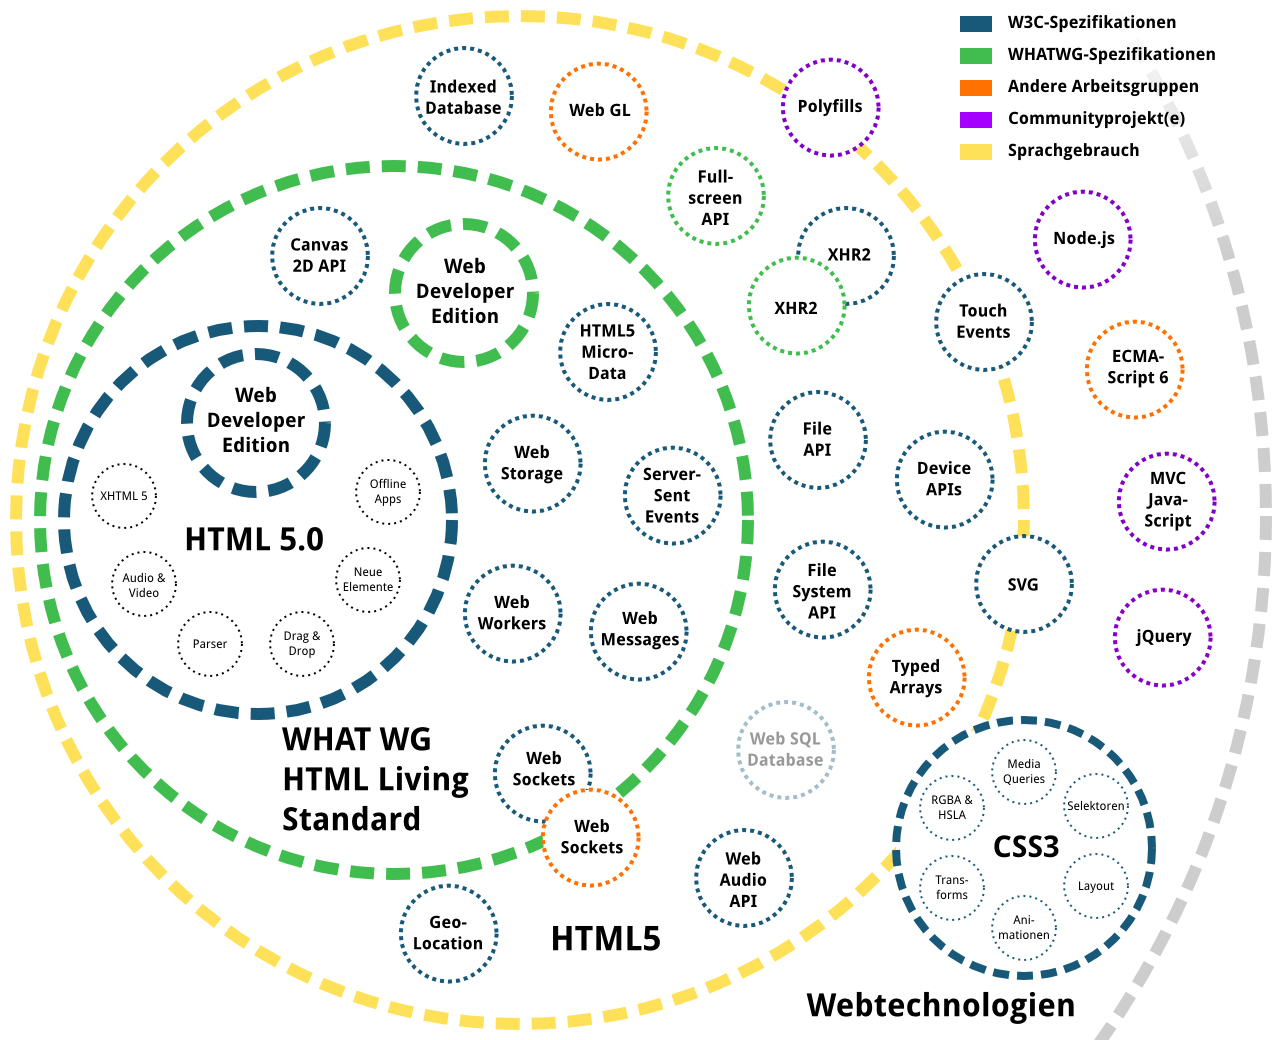
\includegraphics[width=0.87\linewidth]{images/html5_specs.png}
		\captionof{figure}[HTML5 Spezifikationen Übersicht]{HTML5 Spezifikationen Übersicht}
		\label{fig:html5specs}
	\end{minipage}

\paragraph{Ziele} \ac{HTML}5 wurde mit besonderem Augenmerk auf die Kompatibilität entwickelt. Vorhandene Spezifikationen wie \ac{HTML}4.01, \ac{XHTML}1.0 und \ac{DOM}2 sollten unter einem Dach gebündelt werden. Hierdurch wird der vorangegangenen Fragmentierung entgegen gewirkt. Schon vorhandene Inhalte müssen weitestgehend unterstützt werden auch wenn sie nicht zur \ac{HTML}5 Spezifikation gehören. Beispielsweise werden fehlerhaft verschachtelte Elemente trotzdem akzeptiert. \textit{Graceful degradation} ist als ein weiteres Ziel für HTML5 definiert worden und bedeutet soviel wie \glqq Schrittweise Abstufung\grqq{}. Es stellt sicher, dass ein HTML Dokument auch dann verarbeitet wird sollte der verwendete Browser ein bestimmtes benutztes Element nicht unterstützen. Weiter galt für die Spezifikation, dass schon vorhandene Techniken, die weitläufig verbreitet sind, nicht neu entwickelt werden sollten. Stattdessen sollten sie übernommen werden. Dies beruht auf dem Umstand, dass die Browser Hersteller jeweils ihre eigenen Techniken bevorzugen und weiter entwickeln und dadurch auch für ihre Verbreitung sorgen. Evolution statt Revolution stand über den Zielen von HTML5. (X)HTML wurde weiter entwickelt und nicht von Grund auf neu definiert. So ist in Tabelle \ref{tab:html5browserkomp} die zum aktuellen Zeitpunkt verfügbare Unterstützung von HTML5 in den gängigsten Browsern abzulesen.

\vspace{1em}
\begin{table}[!h]
	\centering
	\begin{tabular}{|l|l|c|}
		\hline
		\textbf{Hersteller} & \textbf{Desktop/Mobile} & \textbf{Version}\\
		\hline
		Mozilla & Firefox & 4.0\\
		\hline
		 & Firefox Mobile & 16\\
		\hline
		Google & Chrome & 10\\
		\hline
		 & Chrome Mobile & 25\\
		\hline
		 & Android & 4.0\\
		\hline
		Apple & Safari & 5.1\\
		\hline
		 & Safari iOS & 5.1\\
		\hline
		Microsoft & Internet Explorer & 10\\
		\hline
		 & Windows Phone & 8\\
		\hline
		Opera Software & Opera & 11.64\\
		\hline
		Blackberry & Browser & 10\\
		\hline
	\end{tabular}
	\caption{HTML5 Browserkompatibilität}
	\label{tab:html5browserkomp}
\end{table}

\paragraph{Aufbau} Ein jedes HTML Dokument beginnt mit dem sogenannten \textit{Doctype}. Dieser legt fest mit welcher Syntax das Dokument aufgebaut ist und wie das Dokument vom Browser verarbeitet werden soll. Verschiedene Varianten wie \textit{strict},\textit{transitional} und \textit{frameset} sind in HTML5 nicht vorgesehen. In den Vorgängerversionen musste die Variante jedoch mit angegeben werden um eine eindeutige Interpretation des Dokuments zu gewährleisten. Listing \ref{lst:html401doctype} zeigt die beiden \textit{Doctype} von HTML 4.01 und XHTML 1.0. Durch die Abwärtskompatibilität von HTML5 sind auch diese \textit{Doctype} heute noch gültig und das Dokument wird korrekt vom Parser interpretiert werden.
    
    \vspace{1em}
	\begin{lstlisting}[caption=(X)HTML4.01 \textit{doctype}-Element, label=lst:html401doctype]
<!DOCTYPE HTML PUBLIC "-//W3C//DTD HTML 4.01//EN"
        "http://www.w3.org/TR/html4/strict.dtd">
<!DOCTYPE HTML PUBLIC "-//W3C//DTD HTML 4.01 Transitional//EN"
        "http://www.w3.org/TR/html4/loose.dtd">
<!DOCTYPE HTML PUBLIC "-//W3C//DTD HTML 4.01 Frameset//EN"
        "http://www.w3.org/TR/html4/frameset.dtd">        
<!DOCTYPE html PUBLIC "-//W3C//DTD XHTML 1.0 Strict//EN"
        "http://www.w3.org/TR/xhtml1/DTD/xhtml1-strict.dtd">    
	\end{lstlisting}
	
Listing \ref{lst:html5doctype}	hingegen zeigt das \textit{Doctype} von HTML5. Es wurde enorm gekürzt im Vergleich zu dem \textit{Doctype} von HTML 4.01 und XHTML 1.0. Groß- und Kleinschreibung ist nicht von bedeutung innerhalb des \textit{Doctype}. 

    \vspace{1em}
	\begin{lstlisting}[caption=HTML5 \textit{doctype}-Element, label=lst:html5doctype]
<!DOCTYPE html>
	\end{lstlisting}		
	
Nach dem \textit{Doctype} folgt der restliche Dokument Aufbau in HTML Syntax. Diese teilt sich auf in Elemente und Attribute, die diesen Elementen zugeordnet und mit Werten versehen werden können. Es existieren für die meisten Elemente Start- und Endmarkierungen. Für einige Elemente sind die Start- bzw. Endmarkierungen optional und für einige wiederum verpflichtend in der Dokumentstruktur zu setzen. In Listing \ref{lst:html5basicdoc} sieht man ein valides HTML5 Dokument mit den Mindestanforderungen.(vgl. \cite{KronHTML2011} S.58)

	\vspace{1em}
	\begin{lstlisting}[caption=HTML5 Basis Dokument, label=lst:html5basicdoc]
<!DOCTYPE html>
<html>
 <head>
  <title>Beispiel Seite</title>
 </head>
 <body>
  <h1>Beispiel Seite</h1>
  <p>Dies ist ein <a href="demo.html">einfaches</a> Beispiel.</p>
  <!-- Dies ist ein Kommentar -->
 </body>
</html>
	\end{lstlisting}
	
\paragraph{Wichtige neue Sprachelemente} In HTML5 wurden die Mikrodaten mit aufgenommen. Mit Mikrodaten bietet sich eine weitere Möglichkeit ein HTML Dokument semantisch zu spezifizieren. Metadaten wie z.B. der verwendete Zeichensatz lassen sich so festlegen. Browser und Webseiten können über die Mikrodaten-\ac{API} die gesetzten Werte auslesen und weiter verarbeiten. Auch Suchmaschinen können auf die Metadaten zugreifen, verwenden sie jedoch heutzutage weitestgehend nicht mehr. Aus diesem Grund tragen die Metadaten zwar zur semantischen Struktur des HTML bei, können aber aus Sicht der Suchmaschinenoptimierung getrost vernachlässigt werden.(vgl. \cite{SelfHtml20142}) Weiter kann man bei Mikrodaten davon sprechen, \glqq [...] dass sie auf Name/Werte-Paaren basieren. Jedes Mikordatenvokabular definiert eine Menge benannter Eigenschaften.\grqq{}(vgl. \cite{PilgDurc2011} S.174) Listing \ref{lst:html5meta} zeigt Beispielhaft das \textit{head}-Element eines HTML Dokuments mit vier, darin eingeschlossenen, \textit{meta}-Elementen. Unter anderem wird mit dem ersten \textit{meta}-Element der Zeichensatz näher definiert. Das \textit{meta}-Element mit Namen \textit{viewport}, dient dazu die Skalierung auf Mobilgeräten zu unterdrücken, damit die Seite sich an den \textit{viewport} anpasst.

    \vspace{1em}
	\begin{lstlisting}[caption=HTML5 \textit{meta}-Element, label=lst:html5meta]
<head>
  <meta charset="utf-8">
  <meta name="viewport" content="width=device-width;" />
  <meta name="keywords" content="Lorem ipsum">
  <meta name="author"   content="dolor sem it">
</head>
	\end{lstlisting}
		
Zwei weitere neue Elemente in HTML5 sind das \textit{header}- und \textit{footer}-Element. Zu Zeiten vor HTML5 wurden jene Bereiche einer Website durch \textit{div}-Elemente mit dem \textit{id}- oder \textit{class}-Attribut entsprechend gekennzeichnet. Das ist jetzt nicht mehr nötig durch die beiden neuen Elemente. Üblich ist es im \textit{header}-Element einer Website Komponenten wie das Logo, das Menü und den Titel unterzubringen. Im \textit{footer}-Element dagegen werden Kontakt, Impressum und das Copyright aufgeführt. In Listing \ref{lst:html5header}	 ist die Platzierung des \textit{header}- und \textit{footer}-Elements innerhalb eines \textit{body}-Elements einer Webseite zu sehen.

    \vspace{1em}
	\begin{lstlisting}[caption=HTML5 \textit{header}- und \textit{footer}-Element, label=lst:html5header]
<body>
  <header>
    <img src="logo.gif" alt="logo">
    <h1>Ueberschrift</h1>
  </header>
  <footer>
     <a href="kontakt.html">Kontakt</a>
  </footer>
</body>
	\end{lstlisting}
	
Um ein HTML Dokument nach heutigen Maßstäben korrekt zu strukturieren wurden einige Elemente der Spezifikation hinzugefügt. So lässt sich die Navigation nun mit dem \textit{nav}-Element umschließen wie in Listing \ref{lst:html5struct} ab Zeile 3 zu sehen. \glqq Das \textit{section}-Element repräsentiert einen allgemeinen Abschnitt in einem Dokument oder einer Anwendung. Ein Abschnitt ist in diesem Kontext eine thematische Gruppierung von Inhalten, die üblicherweise unter einer Überschrift stehen. Beispiele für Abschnitte wären Kapitel, die verschiedene Tabs in einem Dialog mit Tabs oder die nummerierten Abschnitte einer wissenschaftlichen Arbeit.[...] Das \textit{article}-Element repräsentiert eine abgeschlossene Einheit in einem Dokument, einer Anwendung oder einer Site, die unabhängig verbreitet oder wiederverwendet werden kann, z.B. in RSS-Feeds. Es könnte beispielsweise ein Forenbeitrag, ein Zeitschriften- oder Zeitungsartikel, ein Blog-Eintrag, ein Benutzerkommentar, ein interaktives Widget oder Gadget oder ein Element mit unabhängigem Inhalt enthalten. Das \textit{aside}-Element repräsentiert einen Abschnitt einer Seite, der Inhalte enthält, die sich zwar auf den das \textit{aside}-Element umgebenden eigentlichen Inhalt der Seite beziehen, aber als von ihm unabhängig betrachtet werden können. In Druckwerken werden derartige Abschnitte häufig als Seitenleisten dargestellt. Das Element kann für typografische Effekte wie herausgehobene Zitate oder Seitenleisten, für Werbung, für Gruppen von \textit{nav}-Elementen und andere Inhalte verwendet werden, die als vom eigentlichen Inhalt der Seite getrennt betrachtet werden können.\grqq{}\cite{PilgDurc2011} Das neue \textit{main}-Element ist zur Auszeichnung des Seitenhauptinhalts vorgesehen. Mit dieser Auszeichnung lässt sich z.B. mit Screenreadern direkt zum Hauptinhalt springen.  Alle genannten Elemente sind in Listing \ref{lst:html5struct} in ihrer vorgesehenen Reihenfolge abgebildet.

    \vspace{1em}
	\begin{lstlisting}[caption=HTML5 Struktur Elemente, label=lst:html5struct]
<body>
  <header>
    <nav>
      <ul>
        <li><a href="#link_1.html">Wiki</a></li>
        ...
      </ul>
    </nav>
  </header>
  <main>
  <article>
    <h1>Ueberschrift</h1>
    <p>Dies ist eine Beispiel HTML5-Seite</p>
  </article>
  <aside>
    <section>
      <h2>Kontakt</h2>
      <ul>
        <li><a href="link_1.html">Wiki</a></li>
        ...
      </ul>
    </section>
  </aside>
  </main>
  <footer>
  </footer>
</body>
	\end{lstlisting}

\glqq Damit auch ältere Internet Explorer der Versionen 6-8 die neuen HTML5-Elemente darstellen können, kann ein kurzes JavaScript eingebunden werden. Am einfachsten ist es, dieses nicht auf dem eigenen Server vor zuhalten, sondern direkt von Google abzurufen. Dies hat überdies den Vorteil, dass es oft schon im Browser-Cache der Nutzer vorhanden ist. Der Aufruf erfolgt in einem \textit{Conditional Comment}, der nur vom Internet Explorer kleiner als Version 9 (lt IE 9) verstanden wird. Alle andere Browser ignorieren dies als reinen Kommentar.\grqq{}\cite{SelfHtml20143} In Listing \ref{lst:html5fallback}	 ist der beschriebene Rückfallmechanismus verdeutlicht.

    \vspace{1em}
	\begin{lstlisting}[caption=HTML5 Internet Explorer Fallback, label=lst:html5fallback]
<head>
  <meta charset="utf-8">
  <!--[if lt IE 9]>
    <script src="//html5shim.googlecode.com/svn/trunk/html5.js"></script>
  <![endif]-->
  <title>HTML5-Seite mit Grundstruktur</title>
</head>
	\end{lstlisting}
	
Eingabefelder sind in den meisten Applikationen unabdingbar. Aus diesem Grund wurden in HTML5 eine vielzahl an \textit{input}-Elementen hinzugefügt. So müssen keine komplizierten Workarounds mit JavaScript oder anderen Skriptsprachen mehr verwendet werden. \glqq Das typische HTML5-Formular unterscheidet sich nicht fundamental von seinen in HTML 4.01 oder XHTML 1 geschriebenen Gegenstücken. Alle alten Formularelemente sind noch da und verhalten sich weitgehend wie bisher. Die Neuerungen bestehen aus einigen neuen Funktionen, Attributen und \ac{API}s und aus einer ganzen Reihe neuer möglicher Werte für das \textit{type}-Attribut des \textit{input}-Elements.\grqq{}\cite{KronHTML2011} In Listing \ref{lst:html5input} sind beispielhaft einige neue Werte des \textit{type}-Attributs ausgeführt. Eingabefelder des Typs \textit{tel, email} oder \textit{url} sind vom Verständnis her simple Texteingabefelder. Als wichtige Besonderheit lässt sich bei \textit{email}- und \textit{url}-Feldern aber ihre eingebaute Validation nennen. Verwendet man die Validierungs-\ac{API} werden nur korrekte URLs bzw. E-Mails zugelassen. Für ein \textit{tel}-Feld gilt dies nicht. Außerdem wird auf Smartphones und Tablet-Geräten die angezeigte Bildschirmtastatur entsprechend des erwarteten Eingabetyps für eine optimale Eingabe angepasst dargestellt.(vgl. \cite{KronHTML2011} S.178) So wird bei einer erwarteten E-Mail Adresse das @-Symbol direkt auf der Bildschirmtastatur als eigene Taste mit angezeigt, was normalerweise nicht der Fall ist. Einige der neuen Elementausprägungen besitzen noch zusätzliche Attribute die die Eingabemöglichkeit weiter einschränken und präzisieren können. Zu sehen in Zeile 5 von Listing \ref{lst:html5input} im \textit{time}-Feld, bei dem die erwartete Zeit von 9:00Uhr bis 17:00Uhr nur einstellbar ist. \textit{input}-Elemente können über das \textit{required}-Attribut außerdem als Pflichtfeld markiert werden.

    \vspace{1em}
	\begin{lstlisting}[caption=HTML5 \textit{input}-Element, label=lst:html5input]
<body>
  <input type="tel">
  <input type="email">
  <input type="url">  
  <input type="time"  min="09:00" max="17:00">
  <input type="date"  required="required">
</body>
	\end{lstlisting}
	
Für multimediale Inhalte auf Webseiten wurden der Spezifikation passende Elemente hinzugefügt. Das \textit{canvas}-Element \glqq [...] stellt eine Fläche zur Verfügung, auf die mittels JavaScript dynamische Bitmap-Grafiken gezeichnet werden können. So lassen sich Animationen erstellen, Diagramme zeichnen, eigene Interface-Elemente kreieren und Videos manipulieren\grqq{}\cite{KronHTML2011} Für Audio und Video Inhalte wurden die gleichnamigen Elemente geschaffen. 
	
\subsection{CSS3}
// Allgemeiner Aufbau - Gestaltungssprache, Kern Element des WWW, Darstellung und Inhalt getrennt, Unterschiedliche Optik je nach Ausgabe Gerät\\
// Syntax - Selektoren, Eigenschaften, Werte, Pseudoklassen\\
// Listing \ref{lst:css3syntax}
	\vspace{1em}
	\begin{lstlisting}[caption=CSS3 Syntax Beispiel, label=lst:css3syntax]
Selektor [, Selektor2, ...]
  {
    Eigenschaft1: Wert1;
    ...
    EigenschaftN: WertN[;]
  }
  /* Kommentar - In eckigen Klammern stehen optionale Angaben */
	\end{lstlisting}

// CSS-Box-Modell - margin, border, padding\\
// Abbildung \ref{fig:cssboxmodell}\\
	\vspace{1em}
	\begin{minipage}{\linewidth}
		\centering
		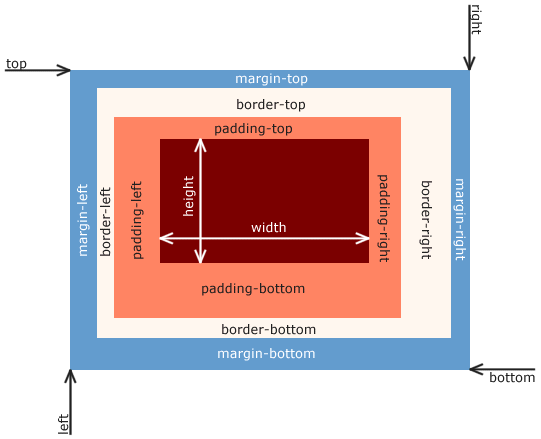
\includegraphics[width=0.7\linewidth]{images/css_boxmodell.png}
		\captionof{figure}[CSS-Boxmodell]{CSS-Boxmodell\footnotemark }
		\label{fig:cssboxmodell}
	\end{minipage}
	\footnotetext{Quelle: \url{http://commons.wikimedia.org/wiki/File:Boxmodell-detail.png}}
	
// Medienspezifische Stylesheets (@media print, screen, ...)\\
// Listing \ref{lst:css3media}
	\vspace{1em}
	\begin{lstlisting}[caption=CSS3 medienspezifisches Stylesheet, label=lst:css3media]
@media print {
	body {
		color: black;
		background-color: white;
	}
	.navigation {
		display: none;
	}
}
	\end{lstlisting}

// Eigenschaftsspezifische Stylesheets (@media screen and (max-width:1024px))\\
// Listing \ref{lst:css3mediaquery}
	\vspace{1em}
	\begin{lstlisting}[caption=CSS3 eigenschaftsspezifisches Stylesheet, label=lst:css3mediaquery]
#inhalt {
	width: 800px;
}
 
@media screen and (max-width: 1024px) {
	#inhalt {
		width: 600px;
	}
 
	aside {
		display: none;
	}
}
	\end{lstlisting}
	
// Verzahnung mit HTML5 - link tag, style tag, html tag, @import innerhalb Stylesheet\\
// Listing \ref{lst:css3einbindunglink} - Einbindung über Link Tag
	\vspace{1em}
	\begin{lstlisting}[caption=Stylesheet Einbindung über \textit{link}-Element, label=lst:css3einbindunglink]
<link rel="stylesheet" type="text/css" href="beispiel.css" />
	\end{lstlisting}
	
// Listing \ref{lst:css3einbindungstyle} - Einbindung über Style Tag
	\vspace{1em}
	\begin{lstlisting}[caption=Stylesheet Einbindung über \textit{style}-Element, label=lst:css3einbindungstyle]
<head>
	<title>Dokument mit Formatierungen</title>
	<style type="text/css">
		body { color: purple; background-color: #d8da3d; }
	</style>
</head>
	\end{lstlisting}
	
// Listing \ref{lst:css3einbindunghtml} - Einbindung in HTML Tag
	\vspace{1em}
	\begin{lstlisting}[caption=Stylesheet Einbindung in \textit{html}-Element, label=lst:css3einbindunghtml]
<span style="font-size: small;">Text</span>
	\end{lstlisting}

\subsection{JavaScript}
// Grundlagen - Geschichte, Sicherheit, aktueller Stand\\
// Listing \ref{lst:jseinbindunghead} - Einbindung als separate Datei im Head
	\vspace{1em}
	\begin{lstlisting}[caption=JavaScript Einbindung als separate Datei im \textit{head}-Element, label=lst:jseinbindunghead]
<script src="script.js" type="text/javascript"></script>
	\end{lstlisting}

// Listing \ref{lst:jseinbindungscript} - Einbindung in Skript Tag im Head und Body
	\vspace{1em}
	\begin{lstlisting}[caption=JavaScript Einbindung in Skript Element im \textit{head}- und \textit{body}-Element, label=lst:jseinbindungscript]
<script type="text/javascript"></script>
	\end{lstlisting}

// Sprachelemente - Kommentare, Funktionen, Objekte\\

// Variablen - Dynamische Typisierung(Loose Typing), Case-Sensitive, ungarische Nomenklatur, spezielle Werte(\textit{undefined, null, true, false, NaN}\\

// Operatoren - \textit{+,-,*,/}, zusätzlich \textit{+} als Zeichenverkettung, In- und Dekrement, Zuweisung, Vergleich, typeof, Logisch\\

// Kontrollstrukturen - \textit{if, switch, for, while} Anweisungen inklusive ihrer Varianten\\

// Document Object Model - Schnittstelle zum HTML Aufbau, W3C Spezifikation unterschieldich implementiert, Knoten Beziehungen, Verarbeitung des DOM, Generierung von HTML durch Serialisierung, Listing \ref{lst:html5beispieltable} beschreiben und zur Baumstruktur hinleiten\\
// Listing \ref{lst:html5beispieltable}
	\vspace{1em}
	\begin{lstlisting}[caption=DOM5 Beispiel Definition, label=lst:html5beispieltable]
<table>
  <thead>
    <tr>
      <th>Vorname</th>
      <th>Name</th>
    </tr>
  </thead>
  <tbody>
    <tr>
      <td>Donald</td>
      <td>Duck</td>
    </tr>
  </tbody>
</table>
	\end{lstlisting}

// Abbildung \ref{fig:dombeispielbaum}\\
	\vspace{1em}
	\begin{minipage}{\linewidth}
		\centering
		
\includegraphics[width=0.5\linewidth]{images/dom_sampletree.png}
		\captionof{figure}[DOM Beispielbaum]{DOM Beispielbaum}
		\label{fig:dombeispielbaum}
	\end{minipage}

// Ereignisse\\
// Übersicht einiger wichtiger Events
    \begin{compactitem}
	    \item onabort (bei Abbruch)
	    \item onblur (beim Verlassen)
	    \item onchange (bei erfolgter Änderung)
	    \item onclick (beim Anklicken)
	    \item ondblclick (bei doppeltem Anklicken)
	    \item onerror (im Fehlerfall)
	    \item onfocus (beim Aktivieren)
	    \item onkeydown (bei gedrückter Taste)
	    \item onkeypress (bei gedrückt gehaltener Taste)
	    \item onkeyup (bei losgelassener Taste)
	    \item onload (beim Laden einer Datei)
	    \item onmousedown (bei gedrückter Maustaste)
	    \item onmousemove (bei weiterbewegter Maus)
	    \item onmouseout (beim Verlassen des Elements mit der Maus)
	    \item onmouseover (beim Überfahren des Elements mit der Maus)
	    \item onmouseup (bei losgelassener Maustaste)
	    \item onreset (beim Zurücksetzen des Formulars)
	    \item onselect (beim Selektieren von Text)
	    \item onsubmit (beim Absenden des Formulars)
	    \item onunload (beim Verlassen der Datei)
    \end{compactitem}

\paragraph{jQuery}
$\;$ \\
// jQuery Bibliothek beinhaltet Elementselektion, Funktionen zum DOM, Animationen und Effekte, AJAX Funktionalitäten\\

// Selektoren\\

// Ereignisse - unterschiede zum JS Standard bei der Definierung, Einfachheit\\

// Übersicht der wichtigsten Funktionen zu Events
    \begin{compactitem}
	    \item .bind – Handler an Event binden
	    \item .on – Handler an Event binden
	    \item .blur – Ereignis, wenn ein Element den Fokus verliert
	    \item .click – Klick mit der Maustaste
	    \item .dbclick – Doppelklick mit der Maustaste
	    \item .hover – Mauszeiger bewegt sich über ein Element
	    \item .mousemove – Mauszeiger bewegt sich in einem Element
	    \item .keypress – eine Taste der Tastatur wird gedrückt
	    \item .keyup – eine Taste der Tastatur wird losgelassen
	    \item .change – ein Formularfeld wird verändert
    \end{compactitem}
    
// DOM-Manipulation\\

// AJAX\\

\subsection{ABAP}
// Herkunft/Entstehung\\
// Grundlagen\\
// Wichtige Elemente (OpenSQL)\\

\subsection{SAP UI5 Framework}
\subsubsection{Definition}
// Aufbauend auf jQuery, AJAX, HTML5/CSS3 \cite{AntoEinf2014}\\

\subsubsection{Architektur}
// Einführung in SAPUI5 S. 123 \cite{AntoEinf2014}\\
// Abbildung \ref{fig:mvcarch}\\
	\vspace{1em}
	\begin{minipage}{\linewidth}
		\centering
		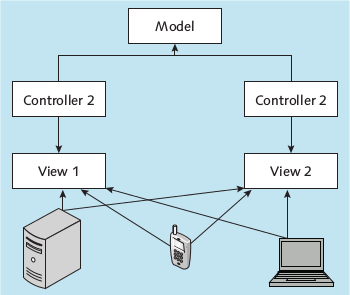
\includegraphics[width=0.6\linewidth]{images/mvc_arch.png}
		\captionof{figure}[Model-View-Controller-Architekturmuster]{Model-View-Controller-Architekturmuster\cite{AntoEinf2014}}
		\label{fig:mvcarch}
	\end{minipage}

\subsubsection{OData Protokoll}
// Einführung in SAPUI5 S. 168 \\
// SAP Netweaver Gateway OData Services\\
\pagebreak

% ----------------------------------------------------------------------------------------------------------
% Kapitel
% ----------------------------------------------------------------------------------------------------------
\section{Software Ergonomie}
// Beleg für die Wichtigkeit von Software Ergonomie\\
// Kurze Übersicht über das Themenfeld Software Ergonomie\\
// Wichtigsten Aspekte nennen und näher erläutern\\

\subsection{Definition}
\paragraph{Kognitionspsychologie}
// Modellierung und Simulation von menschlichen Denk- und Wahrnehmungsprozessen\\

\paragraph{Arbeitsphysiologie, Industrieanthropologie}
// Beschäftigung mit grundlegenden menschlichen Fähigkeiten zur Informationsaufnahme und Informationsverarbeitung\\

\paragraph{Arbeitspsychologie}
// Untersuchung der Wechselbeziehungen zwischen Arbeit, deren Schnittstellen und psychischen Faktoren (unter anderem Arbeitszufriedenheit und -unlust)\\

\subsection{DIN EN ISO 9241}
// DIN Norm zur Software Ergonomie\\
// Die 7 Grundsätze der Dialoggestaltung:
\begin{compactitem}
	\item Aufgabenangemessenheit
	\item Selbstbeschreibungsfähigkeit
	\item Erwartungskonformität
	\item Fehlertoleranz
	\item Steuerbarkeit
	\item Individualisierbarkeit
	\item Lernförderlichkeit
\end{compactitem}
\paragraph{DIN EN ISO 14915}
$\;$ \\
// Erweiterung der ISO 9241\\

\subsection{Analyse Methoden}
\paragraph{Eye Tracking}
// Funktionsweise und Ergebnis\\

\paragraph{Mouse Clicking}
// Funktionsweise und Ergebnis\\

\subsection{SAP Technologien in Bezug auf Software Ergonomie}
\subsubsection{Business Server Pages}
// \ac{BSP} ist old school Technik\\
// geklaut von \ac{JSP}\\

\subsubsection{Web Dynpro for ABAP}
// Aktuelle Technik\\
// ABAP Code generiert HTML\\
// statischer und dynamischer Teil\\

\subsubsection{SAP Fiori / SAP UI5 / SAP Screen Personas}
// cutting edge\\
// aktuelle SAP UI Strategie\\
// SAP Präsi Chart Fiori/SP renew, etc. pp\\
// SAP Fiori einerseits Name des Themes/Guideline\\
// andererseits Bündel der gängigsten TAs/GPs als fertige\\
// Mobile First/Responsive Design Applikationen\\
// SAP UI5 - SAPs Framework zur Entwicklung von eigenen Applikationen im Fiori Style\\
// Nicht zu tief auf JS, HTML etc eingehen, dass kommt im nächsten Kapitel\\
// SAP SP - Zusätzliche Schicht um Standard Dynpro zu Personalisieren und so\\
\pagebreak

% ----------------------------------------------------------------------------------------------------------
% Kapitel
% ----------------------------------------------------------------------------------------------------------
\section{Fallbeispiel SAP UI5}
Lorem ipsum dolor sit amet.

\subsection{Beschreibung}
// Frontend - Browser, Elemente\\
// Backend - JSON, OData Model\\
// Analyse der wichtigen Arbeitsschritte\\

\subsection{Hilfsmittel}
\subsubsection{Entwicklungsumgebung}
// Kurze Beschreibung der Entwicklungsumgebung\\
// Sprich Eclipse, SE80, Chrome Dev-tools, Debugger\\
// Neptune Application Designer\\

\subsubsection{UI Design und Prototyping}
// Wireframing als Prototyping\\
// Abbildung Wireframesketcher\\

\subsection{Implementierung}
\subsubsection{View}
// Auszugsweise Coding bringen um bestimmte Elemente aus der Theorie zu zeigen\\
// Generellen Aufbau der Views erklären\\
// Kapselung wird dadurch verdeutlicht\\
// Listing \ref{lst:app.view.js}
	\vspace{1em}
	\begin{lstlisting}[caption=Root View der Applikation, label=lst:app.view.js]
sap.ui.jsview("abat.Mockup.view.App", {

  getControllerName: function () {
    return "abat.Mockup.view.App";
  },
  
  createContent: function (oController) {
    // to avoid scroll bars on desktop
    this.setDisplayBlock(true);
    
    // create app
    this.app = new sap.m.SplitApp();
    
    // load the master page
    var master = sap.ui.xmlview("Master", "abat.Mockup.view.Master");
    master.getController().nav = this.getController();
    this.app.addPage(master, true);
    
    // load the empty page
    var empty = sap.ui.xmlview("Empty", "abat.Mockup.view.Empty");
    this.app.addPage(empty, false);
    
    // wrap app with shell
    return new sap.m.Shell("Shell", {
      title : "{i18n>ShellTitle}",
      showLogout : false,
      app : this.app
    });
  }
});
	\end{lstlisting}

// Master/Detail Applikation mit Fragment und Chart View Aufbau\\
// TODO: Visio Diagramm oder vergleichbares erstellen\\
// sap.ui.view\\
//   |- sap.m.Shell\\
//   |  |- sap.m.SplitApp\\
//   |  |  |- sap.m.Page\\
//   |  |  |  |- sap.m.Bar\\
//   |  |  |  |- sap.m.Bar\\
//   |  |  |  |- sap.m.List\\
//   |  |  |  |  |- sap.m.ObjectListItem\\
//   |  |  |  |- sap.m.Bar\\
//   |  |  |- sap.m.Page\\
//   |  |  |  |- sap.m.ObjectHeader\\
//   |  |  |  |  |- sap.m.ObjectAttribute\\
//   |  |  |  |  |- sap.m.ObjectAttribute\\
//   |  |  |  |  |- sap.m.ObjectAttribute\\
//   |  |  |  |  |- sap.m.ObjectAttribute\\
//   |  |  |  |  |- sap.m.ObjectStatus\\
//   |  |  |  |- sap.IconTabBar\\
//   |  |  |  |  |- sap.IconTabFilter\\
//   |  |  |  |  |  |- sap.ui.core.Fragment\\
//   |  |  |  |  |  |  |- sap.ui.core.FragmentDefinition\\
//   |  |  |  |  |  |  |  |- sap.viz.ui5.Bar\\
//   |  |  |  |  |- sap.IconTabFilter\\
//   |  |  |  |  |  |- sap.ui.core.Fragment\\
//   |  |  |  |  |  |  |- sap.ui.core.FragmentDefinition\\
//   |  |  |  |  |  |  |  |- sap.viz.ui5.Bar\\
//   |  |  |  |- sap.m.Bar\\


\subsubsection{Model und Controller}
// die Verbindung von beiden Anhand von Coding zeigen\\
// TODO: OData Modell einbinden\\
// Listing \ref{lst:Component.js}
	\vspace{1em}
	\begin{lstlisting}[caption=Component.js - Datenmodell an die Root View binden, label=lst:Component.js]
...
// JSON Modell an die Root View binden
var oModel = new sap.ui.model.json.JSONModel("model/mock.json");
oView.setModel(oModel);

// OData Modell
var oModel = new sap.ui.model.odata.ODataModel(<URL>);
oView.setModel(oModel);

// I18N(Lokalisierung) Modell
var i18nModel = new sap.ui.model.resource.ResourceModel({
  bundleUrl : "i18n/messageBundle.properties"
});
oView.setModel(i18nModel, "i18n");

// Geraetespezifisches Modell
var deviceModel = new sap.ui.model.json.JSONModel({
  isPhone : jQuery.device.is.phone,
  listMode : (jQuery.device.is.phone) ? "None" : "SingleSelectMaster",
  listItemType : (jQuery.device.is.phone) ? "Active" : "Inactive"
});
deviceModel.setDefaultBindingMode("OneWay");
oView.setModel(deviceModel, "device");
...
	\end{lstlisting}

\subsubsection{Backend}
// ABAP Stack der den RESTful Service bereitstellt zeigen\\
// Beispielhafte Implementation des HTTP Responses\\
\pagebreak

% ----------------------------------------------------------------------------------------------------------
% Kapitel
% ----------------------------------------------------------------------------------------------------------
\section{Analyse}
\subsection{Heatmap}
// Angewandte Analyse mit Heatmap\\

\subsection{UI-Objekte}
// Mobile First/Responsive Design\\

\subsection{PLATZHALTER}
// PLATZHALTER\\
\pagebreak

% ----------------------------------------------------------------------------------------------------------
% Kapitel
% ----------------------------------------------------------------------------------------------------------
\section{Schluss}
Lorem ipsum dolor sit amet.

\paragraph{Zusammenfassung}
// Arbeitsgebiete, Produktions \& Dienstleistungsbereiche\\
// Arbeitsergebnisse\\
// Projektziele, Projektergebnisse, Projekttermine\\
// Mitwirkungszeiträume\\
// Liste aller selbst wahrgenommen Aufgaben und Tätigkeiten\\
// Projektmeilensteine\\
// Ablauforganisation \& Beteiligte\\
// Arbeitsformen, Arbeitsmittel, Arbeitsabläufe\\
// Kommunikations- / Informationsgewohnheiten\\
// Auswertung relevanter Literatur\\
// Themen aus Lehrveranstaltungen\\

\paragraph{Bewertung}
// Wesentliche Erkenntnisse und Erfahrungen\\
// Folgerungen und Konsequenzen\\
// Vorschläge für Verbesserung und Veränderung\\
// Auswirkungen auf persönliche Berufs- und Karriereplanung\\
// Bezug zum Studium\\
// hilfreiche Studieninhalte\\
// neu gewonnenes Interesse\\
\pagebreak

% ----------------------------------------------------------------------------------------------------------
% Literatur
% ----------------------------------------------------------------------------------------------------------
\renewcommand\refname{Quellenverzeichnis}
\bibliographystyle{myalpha}
\bibliography{bibo}
\pagebreak

% ----------------------------------------------------------------------------------------------------------
% Anhang
% ----------------------------------------------------------------------------------------------------------
\pagenumbering{Roman}
\setcounter{page}{1}
\lhead{Anhang \thesection}

\begin{appendix}
\section*{Anhang}
\phantomsection
\addcontentsline{toc}{section}{Anhang}
\addtocontents{toc}{\vspace{-0.5em}}

\section{GUI}
Ein toller Anhang.

\subsection*{Screenshot}
\label{app:screenshot}
Unterkategorie, die nicht im Inhaltsverzeichnis auftaucht.

\end{appendix}

\newpage
\thispagestyle{empty}
\begin{center}
	\vspace*{5em}
	\huge\textbf{Erklärung}\\
\end{center}
\vspace{2em}
Hiermit versichere ich, dass ich meine Abschlussarbeit selbständig verfasst und keine anderen als die angegebenen Quellen und Hilfsmittel benutzt habe.

\vspace{4em}
\begin{minipage}{\linewidth}
	\begin{tabular}{p{15em}p{15em}}
		Datum: &  .......................................................\\
		& \centering (Unterschrift)\\
	\end{tabular}
\end{minipage}

\end{document}
